\documentclass[glossy]{beamer}
\useoutertheme{wuerzburg}
\useinnertheme[realshadow,corners=2pt,padding=2pt]{chamfered}
\usecolortheme{shark}

\usepackage{listings}
\usepackage[utf8]{inputenc}


\usepackage{fancyvrb}
%\usepackage[scaled]{beramono} %sets the beramono font. Just comment this line to get the default font back

\usepackage{tikz}
\newcommand<>{\hover}[1]{\uncover#2{%
 \begin{tikzpicture}[remember picture,overlay]%
 \draw[fill,opacity=0.4] (current page.south west)
 rectangle (current page.north east);
 \node at (current page.center) {#1};
 \end{tikzpicture}}
}

\title{Arquitecturas y Organización de Computadoras I \\\line(1,0){320}}
% \author{\texorpdfstring{Author\newline\url{email@email.com}}{Author}}
%\author{Rafael Ignacio Zurita}
\institute{Rafael Ignacio Zurita \\ Departamento de Ingenieria de Computadoras - FAI - UNCOMA 2018 \\ Clase presencial 8}
%\date{\today}



\begin{document}




\begin{frame}
\maketitle
\end{frame}

\institute{Departamento de Ingenieria de Computadoras - FAI - UNCOMA \\ 2018}

\begin{frame}
\frametitle{Programa Analítico}
\textbf{UNIDAD 2: Unidad Central de Proceso}
 \\~\\
Introducción al diseño lógico. Tablas de verdad. Álgebra de Boole.  Circuitos  combinacionales.  Relojes.  Elementos  de memoria.  Flip-flops,  cerrojos (latches) .  Circuitos  secuenciales.  Implementación de FSM. Circuitos lógicos programables. Unidad Lógica aritmética. Implementación de la suma, resta y operaciones lógicas.  Concepto  de  máquinas  algorítmicas.  \textbf{Camino  de  datos.  Unidad  de  control.}  Implementación  del  algoritmo    básico  de multiplicación. Conceptos de representación de número en punto flotante y error. Suma y multiplicación de punto flotante.
 \\~\\
\end{frame}


\begin{frame}
\frametitle{Temario}
\textbf{UNIDAD 2 - Máquinas Algorítmicas de propósito general \\ Unidad Central de Proceso}
\begin{itemize}
\item Circuitos combinacionales y secuenciales necesarios
\item Camino de datos de un sólo ciclo
\item Camino de datos multiciclo
\item \textbf{Camino de datos segmentado}
\end{itemize}
\end{frame}




\begin{frame}
\frametitle{Temario}
        \begin{center}
        \textbf{Microarquitectura}
        \end{center}
\begin{tabular}{cl}

\begin{tabular}{c}
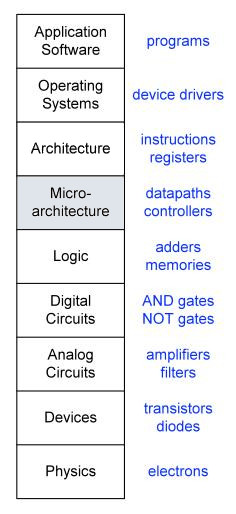
\includegraphics[height=6cm, width=4cm]{estructura-por-niveles.jpg} 

\end{tabular}
& \begin{tabular}{l}
\parbox{0.5\linewidth}{
        Como implementar una arquitectura en hardware (meta: costo, rendimiento, etc) \\ \\
        La microarquitectura es construída por circuitos lógicos y elementos de memoria \\ \\
        Todos los circuitos lógicos y elementos de memoria son implementados físicamente con transistores
}
\end{tabular} \\

\end{tabular}
\end{frame}





\begin{frame}
\frametitle{Implementación de la Microarquitectura}
\begin{center}\textbf{Diseño de la Microarquitectura (diseño del procesador)}\end{center}
\begin{enumerate}
\item Analizar el conjunto de instrucciones (ISA)
\begin{itemize}
\item Obtener los requerimientos del camino de datos
\end{itemize}
\item Seleccionar los \textit{componentes} y establecer la \textit{metodología} del reloj
\item Componer el \textit{camino de datos} para cumplir los requerimientos
\item Determinar las \textit{señales de control} para cada instrucción
\item Componer la \textit{lógica de control (unidad de control)} para generar las señales de control
\end{enumerate}
\end{frame}



\begin{frame}
\frametitle{Implementación de la Microarquitectura}
\begin{center}\textbf{Microarquitectura segmentada }\end{center}
\begin{itemize}
\item Uso de varias unidades al mismo
\item Compartir elementos entre diferentes instrucciones
\item \textbf{Paralelismo a nivel de instrucciones}
\end{itemize}
\end{frame}




\begin{frame}
\frametitle{Implementación de la Microarquitectura}
\begin{center}\textbf{Ejemplo de la lavandería}\end{center}
\begin{itemize}
\item Problema de trabajo
\begin{itemize}
\item Cuatro etapas de tareas
\item Tiempos balanceados (aprox. 30 min.)
\item Secuencia fija de pasos
\item Tiempo total para n trabajos = (n * 2hs.)
\end{itemize}
\end{itemize}
\begin{figure}
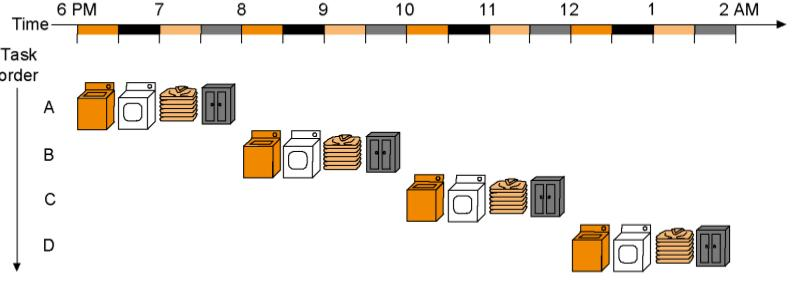
\includegraphics[scale=0.4]{lavanderia1.jpg} 
\end{figure}
\end{frame}




\begin{frame}
\frametitle{Implementación de la Microarquitectura}
\begin{center}\textbf{Ejemplo de la lavandería}\end{center}
\begin{itemize}
\item Optimizacion real
\begin{itemize}
\item Las unidades operan independientemente
\item Se pueden utilizar unidades al mismo tiempo
\item Tiempo promedio por lavado similar al anterior
\item Tiempo total para n cargas = aprox. (n * tiempo por etapa)
\end{itemize}
\end{itemize}
\begin{figure}
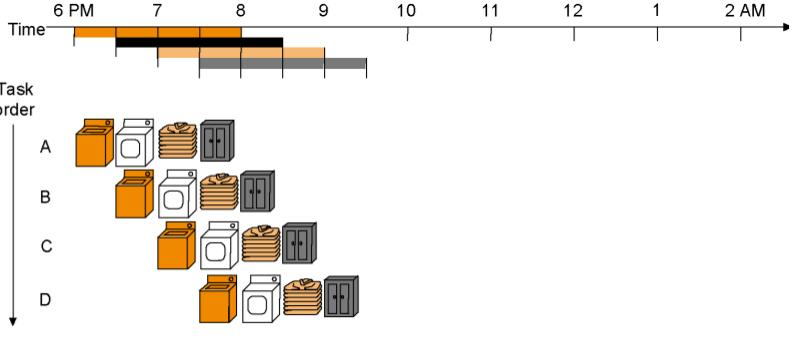
\includegraphics[scale=0.4]{lavanderia2.jpg} 
\end{figure}
\end{frame}




\begin{frame}
\frametitle{Implementación de la Microarquitectura}
\begin{center}\textbf{Tiempo del camino segmentado}\end{center}
\begin{itemize}
\item Ciclo único vs. ejecución segmentada
\end{itemize}
\begin{figure}
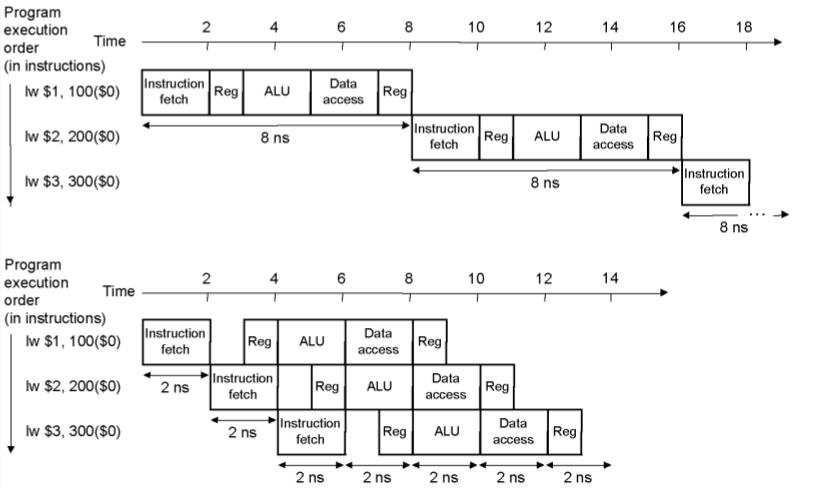
\includegraphics[scale=0.35]{singlevspipelined.jpg} 
\end{figure}
\end{frame}


\begin{frame}
\frametitle{Implementación de la Microarquitectura}
\begin{center}\textbf{Precondiciones}\end{center}
\begin{itemize}
\item Diseño del conjunto de instrucciones
\begin{itemize}
\item Instrucciones de ancho fijo (idealmente)
\item Pocos formatos de instrucciones
\item Operandos en memoria sólo para instrucciones de carga y almacenamiento
\item Datos alineados
\end{itemize}
\end{itemize}
\begin{itemize}
\item Origen de los problemas
\begin{itemize}
\item Instrucciones con longitud variable
\item Datos no alineados
\end{itemize}
\end{itemize}

\end{frame}








\begin{frame}
\frametitle{Implementación de la Microarquitectura}
\begin{center}\textbf{Camino de datos de un ciclo}\end{center}
\begin{figure}
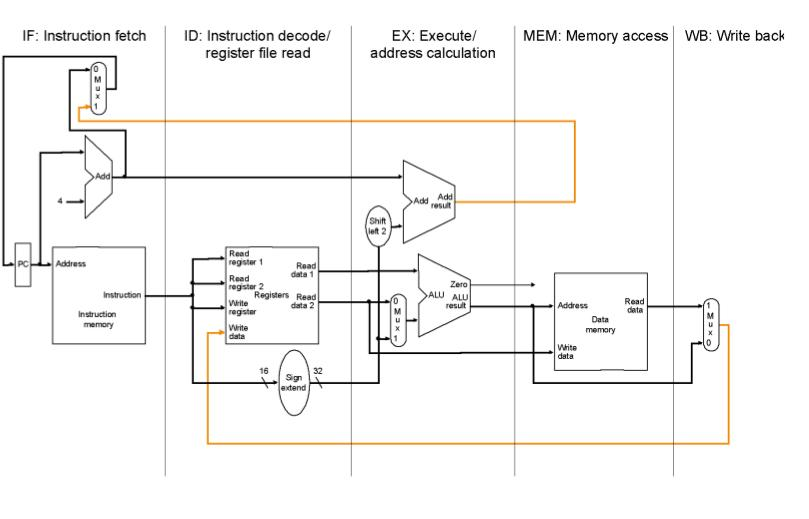
\includegraphics[scale=0.3]{single.jpg} 
\end{figure}

\end{frame}




\begin{frame}
\frametitle{Implementación de la Microarquitectura}
\begin{center}\textbf{Camino de datos segmentado}\end{center}
\begin{figure}
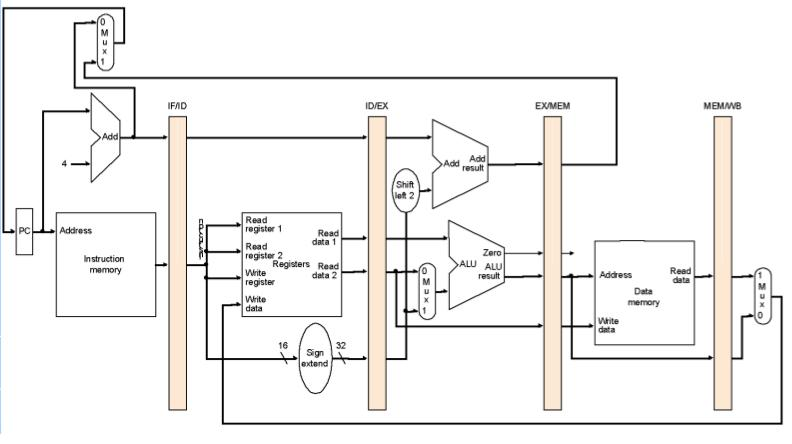
\includegraphics[scale=0.3]{pipelined.jpg} 
\end{figure}

\end{frame}



\begin{frame}
\frametitle{Implementación de la Microarquitectura}
\begin{center}\textbf{Camino de datos segmentado}\end{center}
\begin{itemize}
\item Idea clave: aumentar la productividad (no la latencia)
\item Hardware mas complejo: registros de la microarquitectura
\item Posibilita un incremento de la frecuencia del reloj
\end{itemize}

\end{frame}






\begin{frame}
\frametitle{Implementación de la Microarquitectura}
\begin{center}\textbf{Ejemplo con una única instruccion: lw}\end{center}
\begin{itemize}
\item PC es calculado en la primera etapa
\end{itemize}
\begin{figure}
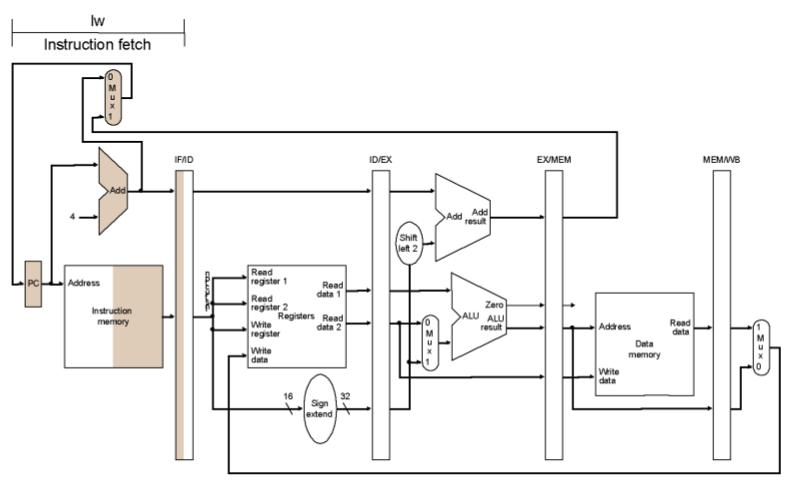
\includegraphics[scale=0.3]{lw1.jpg} 
\end{figure}

\end{frame}



\begin{frame}
\frametitle{Implementación de la Microarquitectura}
\begin{center}\textbf{Ejemplo con una única instruccion: lw}\end{center}
\begin{itemize}
\item Decodificar la instrucción
\item Leer datos del archivo de registros
\end{itemize}
\begin{figure}
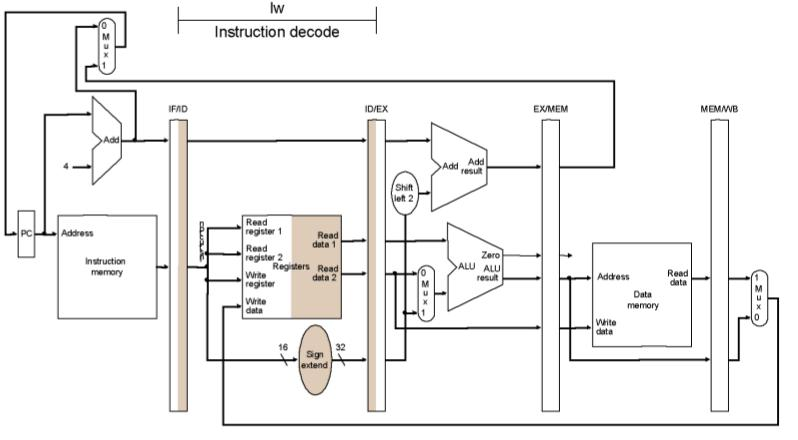
\includegraphics[scale=0.3]{lw2.jpg} 
\end{figure}

\end{frame}




\begin{frame}
\frametitle{Implementación de la Microarquitectura}
\begin{center}\textbf{Ejemplo con una única instruccion: lw}\end{center}
\begin{itemize}
\item Calculo de la dirección efectiva
\end{itemize}
\begin{figure}
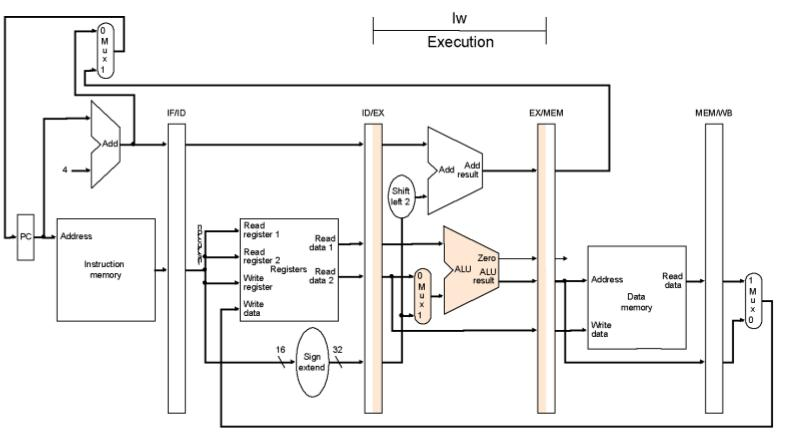
\includegraphics[scale=0.3]{lw3.jpg} 
\end{figure}

\end{frame}

\begin{frame}
\frametitle{Implementación de la Microarquitectura}
\begin{center}\textbf{Ejemplo con una única instruccion: lw}\end{center}
\begin{itemize}
\item Acceso a la memoria de datos
\end{itemize}
\begin{figure}
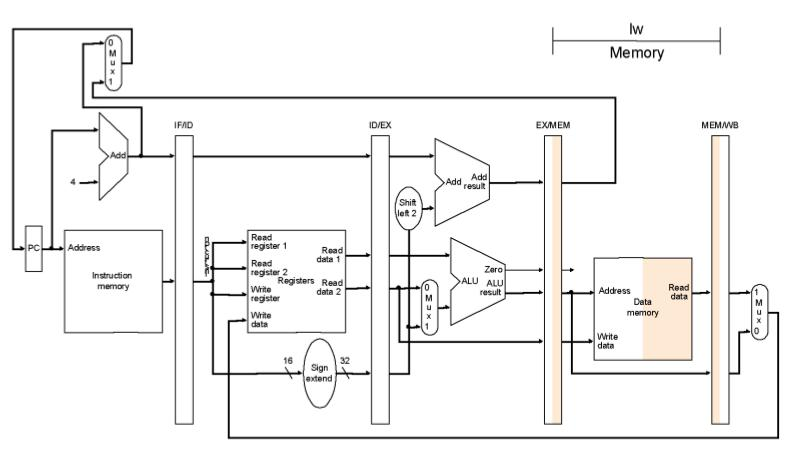
\includegraphics[scale=0.3]{lw4.jpg} 
\end{figure}

\end{frame}

\begin{frame}
\frametitle{Implementación de la Microarquitectura}
\begin{center}\textbf{Ejemplo con una única instruccion: lw}\end{center}
\begin{itemize}
\item Escritura del dato en el archivo de registros
\end{itemize}
\begin{figure}
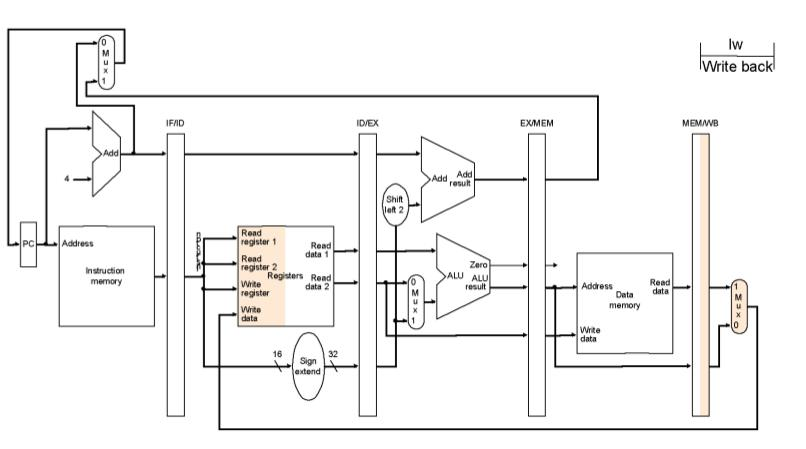
\includegraphics[scale=0.3]{lw5.jpg} 
\end{figure}

\end{frame}







\begin{frame}
 \frametitle{Consejos y preguntas}
\begin{center}
\begin{itemize}
\item  ¿Preguntas?
\end{itemize}
\end{center}
\end{frame}


\begin{frame}
 \frametitle{Bibliografía}
Libros
\begin{itemize}
\item David. Patterson John L. Hennessy (1995), ORGANIZACIÓN Y DISEÑO DE COMPUTADORES La interfaz hardware/software, McGraw-Hill (8 copias en biblioteca).
\end{itemize}
\end{frame}


\end{document}
